% TunnelForge: self-contained Overleaf source.
% Compiler: pdfLaTeX. No external images, bibliography files, or shell escape.
% Original measurements: 29 October 2026. Layout revision: 3 November 2026.
% Do not present loopback results as WAN/TLS or public-cloud measurements.
\documentclass[conference,letterpaper]{IEEEtran}

\usepackage[T1]{fontenc}
\usepackage{amsmath,amssymb}
\usepackage{booktabs,array,tabularx}
\usepackage{graphicx}
\usepackage{cite}
\usepackage{xcolor}
\usepackage{tikz}
\usetikzlibrary{arrows.meta,positioning,fit,backgrounds,calc}
\usepackage{pgfplots}
\pgfplotsset{compat=1.18}
\usepackage{microtype}
\usepackage{url}
\usepackage[hidelinks]{hyperref}
\urlstyle{same}

% Use plain labels instead of IEEEtran's automatically inserted long dashes.
\renewenvironment{abstract}
  {\small\bfseries\noindent Abstract: \ignorespaces}
  {\par\smallskip}
\renewenvironment{IEEEkeywords}
  {\small\noindent\textit{Index Terms: }\ignorespaces}
  {\par\smallskip}

% Preserve IEEEtran's margins and body type size. Avoid geometry and caption
% packages, which can silently override the conference layout.
\newcolumntype{Y}{>{\raggedright\arraybackslash}X}
\newcommand{\KiB}{\,\mathrm{KiB}}
\newcommand{\MiB}{\,\mathrm{MiB}}
\newcommand{\code}[1]{\texttt{#1}}
\definecolor{relayblue}{HTML}{164B75}
\definecolor{palegray}{HTML}{F3F5F7}
\definecolor{darkgray}{HTML}{424242}
\tikzset{
  component/.style={draw=black,rounded corners=2pt,fill=palegray,
    align=center,font=\small,minimum height=12mm,text width=29mm,
    inner sep=4pt,line width=.65pt},
  statebox/.style={draw=black,fill=white,align=center,font=\footnotesize,
    minimum height=10mm,text width=30mm,inner sep=4pt},
  flow/.style={-{Latex[length=2mm,width=1.4mm]},line width=.75pt},
  control/.style={flow,dashed},
  msg/.style={font=\footnotesize,fill=white,inner sep=2pt,align=center},
  lifeline/.style={densely dashed,draw=black!55,line width=.5pt}
}

\begin{document}

\title{TunnelForge: Design and Experimental Evaluation\\
of a Go-Based Reverse HTTP Tunnel over WebSocket}

\author{
\IEEEauthorblockN{Soham Agarwal (202452332), Prem Sharma (202452328),
Aghnivesh Thottumkara (202451175)}
\IEEEauthorblockA{Department of Information Technology\\
Indian Institute of Information Technology\\
\textit{Under the supervision of Dr. Rishabh Gupta}}
}
\maketitle

\begin{abstract}
Demonstrating a local web application to an external caller requires a reachable
endpoint and a mechanism for forwarding requests across network boundaries.
This paper presents TunnelForge, a Go-based reverse HTTP tunnel that carries
structured request and response messages over an outbound WebSocket connection.
The implementation combines temporary registration, token authentication,
ownership-aware request correlation, bounded concurrency, cancellation, and
connection recovery within a single-relay architecture. We evaluate functional
behavior and compare direct HTTP with tunnelled HTTP in a reproducible,
closed-loop experiment. Across 9,216 measured requests with 1~KiB and 64~KiB
payloads, all responses matched the submitted bytes and no request failed.
With one outstanding request, median tunnel latency was 0.182~ms and 3.016~ms,
respectively, compared with 0.035~ms and 0.076~ms for direct HTTP. These
single-machine loopback measurements characterize local implementation overhead,
not Internet performance. The findings illustrate the trade-off between an
inspectable JSON protocol and the processing and buffering costs of a compact
educational tunnel.
\end{abstract}

\begin{IEEEkeywords}
reverse HTTP tunnel, WebSocket, Go, request correlation, concurrency,
developer tools, experimental evaluation
\end{IEEEkeywords}

\section{Introduction}
Local development environments commonly host web interfaces, REST APIs, and
webhook receivers on loopback addresses. These services are convenient for
development but do not automatically provide an endpoint that a remote
collaborator or external webhook provider can reach. Inbound port forwarding,
public deployment, and reverse tunnelling are possible responses. A reverse
tunnel changes the direction of connection establishment: an agent near the
application connects outward to a reachable relay, which forwards incoming
requests over the established channel.

WebSocket provides a persistent bidirectional connection after an HTTP opening
handshake~\cite{websocket}. Selecting that transport does not itself solve HTTP
forwarding. The application must represent HTTP data, correlate out-of-order
responses, manage disconnected peers, serialize socket writes, and terminate
abandoned work. Intermediary behavior must also account for status codes,
header multiplicity, and redirects~\cite{http}.

TunnelForge addresses these concerns using a relay, a command-line client, and
an application that remains an ordinary local HTTP service. The client
authenticates and obtains a temporary routing identifier. The relay converts
incoming requests into JSON messages, and the client reconstructs them for the
local application. Responses return with the original request identifier.
Throughout this paper, \emph{public-side} refers to the relay-facing interface;
the measured deployment is local and does not demonstrate Internet reachability.

The study investigates three questions:

\noindent\textbf{RQ1:} Does the implementation preserve the tested request and
response properties, including arbitrary body bytes?

\noindent\textbf{RQ2:} Do concurrent execution and failure handling maintain request
ownership and release abandoned work?

\noindent\textbf{RQ3:} How does the tunnel change latency and throughput relative to
direct HTTP under controlled local workloads?

The contribution is a reproducible implementation study, rather than a claim
that reverse tunnelling is a new networking technique.

\section{Background and Related Work}
The ngrok documentation describes public endpoints for localhost services,
including webhook testing and traffic inspection use cases~\cite{ngrok}. The
open-source frp project offers a client/server reverse proxy with broader
protocol support and configurable forwarding features~\cite{frp}. These systems
demonstrate the practical relevance of the problem. They are architectural
reference points, not performance baselines here: controlled measurements of
their deployments were not collected.

TunnelForge exposes the mechanism in a smaller codebase: a single relay, an
in-memory registry, a Go client, and explicit message types. It emphasizes
inspectability, constrained HTTP forwarding, and repeatable demonstrations of
concurrency and failure recovery. It does not provide the operational breadth
of a managed gateway or a multi-protocol proxy.

JSON supplies a structured interchange format~\cite{json}; Base64 represents
arbitrary octets using text~\cite{base64}. Go's \code{encoding/json} package
represents byte slices as Base64 strings~\cite{gojson}. These building blocks
make messages easy to inspect, but introduce representation and processing costs
that motivate RQ3. The experiment measures the entire forwarding path and does
not isolate one encoding operation.

\section{System Model and Design}
\subsection{Components and Deployment Assumptions}
The system contains four logical roles: an HTTP caller, the relay, the tunnel
client, and the local application. Fig.~\ref{fig:architecture} separates their
responsibilities and shows the relay's two principal state structures. The
client initiates the WebSocket connection, so the application host need not
accept a separate inbound connection from the relay. Actual remote access still
requires a reachable relay and a network that permits the outbound connection.
NAT traversal is an architectural motivation, not a measured loopback result.

% Wide diagrams use normal 9 to 10 pt labels rather than shrinking an image.
\begin{figure*}[!t]
\centering
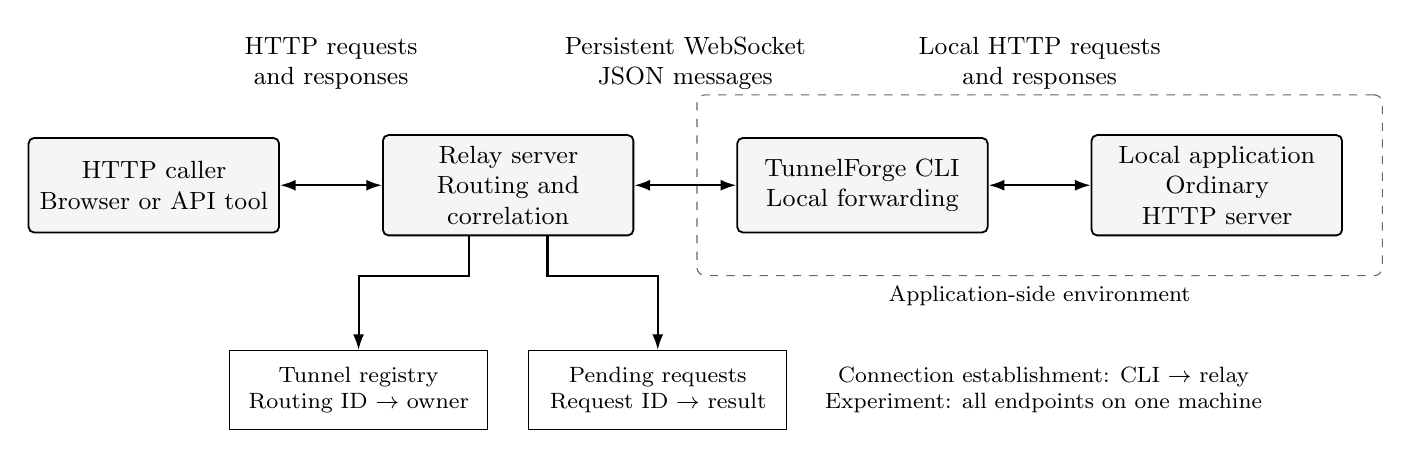
\begin{tikzpicture}[x=1cm,y=1cm,
  channel/.style={{Latex[length=2mm,width=1.4mm]}-{Latex[length=2mm,width=1.4mm]},line width=.75pt}]
  \node[component] (caller) at (0,0) {HTTP caller\\Browser or API tool};
  \node[component] (relay) at (4.5,0) {Relay server\\Routing and correlation};
  \node[component] (cli) at (9,0) {TunnelForge CLI\\Local forwarding};
  \node[component] (app) at (13.5,0) {Local application\\Ordinary HTTP server};
  % Keep labels above the boxes instead of squeezing them into narrow gaps.
  \node[font=\small,align=center] at (2.25,1.55)
    {HTTP requests\\and responses};
  \node[font=\small,align=center] at (6.75,1.55)
    {Persistent WebSocket\\JSON messages};
  \node[font=\small,align=center] at (11.25,1.55)
    {Local HTTP requests\\and responses};
  \draw[channel] (caller.east) -- (relay.west);
  \draw[channel] (relay.east) -- (cli.west);
  \draw[channel] (cli.east) -- (app.west);
  \node[statebox] (registry) at (2.6,-2.6) {Tunnel registry\\Routing ID $\rightarrow$ owner};
  \node[statebox] (pending) at (6.4,-2.6) {Pending requests\\Request ID $\rightarrow$ result};
  \draw[flow] ([xshift=-5mm]relay.south) -- ++(0,-.5) -| (registry.north);
  \draw[flow] ([xshift=5mm]relay.south) -- ++(0,-.5) -| (pending.north);
  \node[font=\footnotesize,align=center] at (11.3,-2.6)
    {Connection establishment: CLI $\rightarrow$ relay\\
     Experiment: all endpoints on one machine};
  \begin{scope}[on background layer]
    \node[draw=black!60,dashed,rounded corners=3pt,
      fit=(cli)(app),inner sep=5mm,
      label={[font=\footnotesize]below:Application-side environment}] {};
  \end{scope}
\end{tikzpicture}
\caption{Logical architecture. The CLI establishes an outbound connection to
the relay. Both directions carry application messages over that connection.
Registry and pending-request state exist only in the relay process.}
\label{fig:architecture}
\end{figure*}

The relay exposes \code{/tunnels} for registration and \code{/health} and
\code{/ready} for process availability. Path routing associates
\code{/t/<identifier>/...} with a connected client, then removes that prefix.
Subdomain routing is also implemented, but needs appropriate DNS and TLS
configuration outside the evaluated environment. The local application does
not import the tunnel protocol.

The registry maps a routing identifier to a tunnel record and connection owner.
Public routing identifiers use five random bytes rendered as hexadecimal;
internal tunnel and request identifiers use sixteen random bytes. Registration
retries on a collision. Random names reduce predictability but do not replace
access control. Disconnecting a client removes its registry entries and cancels
its pending requests. A relay restart discards all active tunnel state.

\subsection{Protocol Representation}
Each message has \code{version}, \code{type}, an optional \code{request\_id},
and a typed \code{payload}. Strict decoding rejects unsupported versions,
unknown types or JSON fields, missing required values, and invalid payload
shapes. Table~\ref{tab:protocol} lists the messages. Connection-scoped messages
manage registration and liveness; request-scoped messages identify independent
exchanges sharing one socket.

\begin{table}[!t]
\caption{Application Protocol Messages}
\label{tab:protocol}
\centering\small
\setlength{\tabcolsep}{4pt}
\begin{tabularx}{\columnwidth}{@{}p{.29\columnwidth}Y@{}}
\toprule
\textbf{Type} & \textbf{Scope and purpose}\\
\midrule
\code{register} & Connection: submit authentication token.\\
\code{registered} & Connection: return tunnel ID and URL.\\
\code{http\_request} & Request: method, path, query, headers, body.\\
\code{http\_response} & Request: status, headers, body.\\
\code{cancel} & Request: cancel the local HTTP context.\\
\code{heartbeat} & Connection: application liveness message.\\
\code{error} & Connection: registration or protocol failure.\\
\bottomrule
\end{tabularx}
\end{table}

Request payloads contain method, path, query, multi-valued headers, and body
bytes. Responses contain status, multi-valued headers, and body bytes. Decoding
reconstructs native Go values before an HTTP exchange is performed locally.
This is application-layer reconstruction, not byte-for-byte preservation of
the original HTTP wire representation. The local target host is configured
explicitly; the original relay-facing host is supplied as forwarding metadata.

\subsection{Binary Data and Representation Cost}
Byte slices avoid assuming valid UTF-8 in HTTP bodies. Base64 preserves their
octets during JSON transport~\cite{gojson}. For a non-empty body of $B$ bytes,
the encoded body length, excluding the JSON envelope and WebSocket framing, is
\begin{equation}
 L(B)=4\left\lceil\frac{B}{3}\right\rceil.
 \label{eq:base64}
\end{equation}
Consequently, 1,024 bytes become 1,368 characters and 65,536 bytes become 87,384
characters. The approximately one-third expansion applies in both directions
for an echoed body. It is a deterministic representation cost, while measured
latency also includes copying, parsing, scheduling, and socket I/O. Bodies are
limited to $1\MiB$ and WebSocket messages to $2\MiB$; headers and envelope fields
consume part of the message allowance.

\subsection{Request Ownership Invariant}
Before dispatch, the relay allocates a pending entry binding a request ID to its
tunnel ID, result channel, and cancellation function. Let $P[r]$ be that entry
and $t$ the responding tunnel. Acceptance requires
\begin{equation}
 \operatorname{accept}(t,r)
 \iff r\in\operatorname{dom}(P)\ \land\ P[r].\operatorname{owner}=t.
 \label{eq:ownership}
\end{equation}
Resolution removes the entry and produces one terminal result. Timeouts,
caller cancellation, and disconnects also terminate pending work. The ownership
check prevents a different connection from completing another tunnel's request,
even if it learns that request ID. It is one specific isolation property, not
a complete multi-tenant authorization system.

\section{Implementation and Failure Handling}
\subsection{End-to-End Forwarding}
The public handler identifies the tunnel, reads the bounded request body,
allocates a pending request, and enqueues its message. The client decodes the
message and invokes the local application. It reads the bounded response and
returns it with the original ID. The relay checks ownership, restores the
tested end-to-end headers, writes the status, and returns the bytes.
Fig.~\ref{fig:sequence} distinguishes this successful path from cancellation.

\begin{figure*}[!t]
\centering
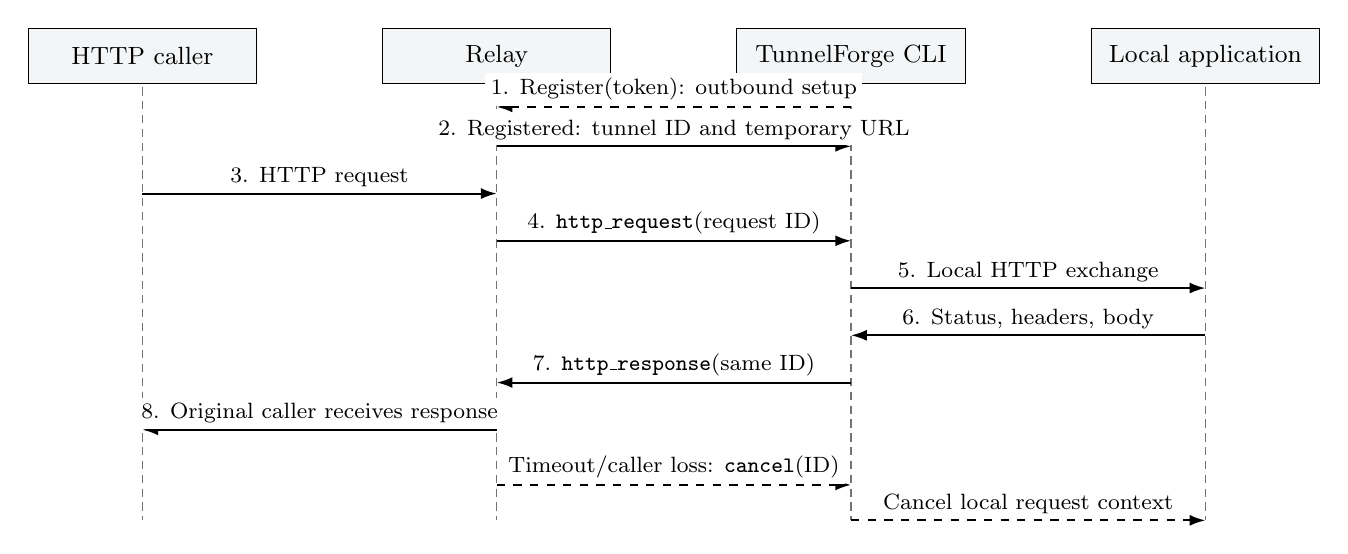
\begin{tikzpicture}[x=1cm,y=1cm]
  \foreach \x/\who in {0/HTTP caller,4.5/Relay,9/TunnelForge CLI,13.5/Local application}{
    \node[draw,fill=palegray,minimum width=29mm,minimum height=7mm,
      font=\small] at (\x,0) {\who};
    \draw[lifeline] (\x,-.4) -- (\x,-5.9);
  }
  \draw[control] (9,-.65) -- node[msg,above]{1. Register(token): outbound setup} (4.5,-.65);
  \draw[flow] (4.5,-1.15) -- node[msg,above]{2. Registered: tunnel ID and temporary URL} (9,-1.15);
  \draw[flow] (0,-1.75) -- node[msg,above]{3. HTTP request} (4.5,-1.75);
  \draw[flow] (4.5,-2.35) -- node[msg,above]{4. \code{http\_request}(request ID)} (9,-2.35);
  \draw[flow] (9,-2.95) -- node[msg,above]{5. Local HTTP exchange} (13.5,-2.95);
  \draw[flow] (13.5,-3.55) -- node[msg,above]{6. Status, headers, body} (9,-3.55);
  \draw[flow] (9,-4.15) -- node[msg,above]{7. \code{http\_response}(same ID)} (4.5,-4.15);
  \draw[flow] (4.5,-4.75) -- node[msg,above]{8. Original caller receives response} (0,-4.75);
  \draw[control] (4.5,-5.45) -- node[msg,above]{Timeout/caller loss: \code{cancel}(ID)} (9,-5.45);
  \draw[control] (9,-5.9) -- node[msg,above]{Cancel local request context} (13.5,-5.9);
\end{tikzpicture}
\caption{Registration, request forwarding, and response correlation. The final
two dashed arrows show an alternative failure branch, not extra steps after a
successful response. Cancellation cannot undo application side effects.}
\label{fig:sequence}
\end{figure*}

Hop-by-hop headers and headers named by \code{Connection} are removed. Header
value lists retain repeated \code{Set-Cookie} fields. Redirect following is
disabled in the local HTTP client so that a 302 is not replaced by a subsequent
response. Automatic decompression is disabled to preserve the upstream
representation. These choices preserve the tested intermediary behavior
associated with HTTP semantics~\cite{http}; complete HTTP conformance is not
asserted.

\subsection{Concurrency and Resource Bounds}
Goroutines serve local requests, while a semaphore permits at most 64 active
exchanges per client connection. Exhausting admission returns 503 instead of
waiting indefinitely for a slot. A mutex serializes client writes. Each relay
socket has one writer pump and a 128-entry outgoing queue. This respects
Gorilla WebSocket's restriction to one concurrent application reader and one
concurrent application writer~\cite{gorilla}.

The relay limits its pending map to 1,000 entries.
Table~\ref{tab:limits} summarizes the configured bounds. They reduce unbounded
growth but do not impose a strict whole-process memory ceiling: body buffers,
JSON copies, headers, queues, and transient allocations also consume memory.
The performance experiment uses at most 32 closed-loop callers, so it evaluates
matching below the 64-request client limit rather than saturation behavior.

\begin{table}[!t]
\caption{Implemented Resource and Timing Limits}
\label{tab:limits}
\centering\small
\setlength{\tabcolsep}{4pt}
\begin{tabularx}{\columnwidth}{@{}Yr@{}}
\toprule
\textbf{Parameter} & \textbf{Value}\\
\midrule
HTTP body / WebSocket message & 1 MiB / 2 MiB\\
Active local requests per connection & 64\\
Pending requests / outgoing queue & 1,000 / 128\\
Relay / local HTTP timeout & 30 s / 35 s\\
Application heartbeat / relay ping & 20 s / 25 s\\
Read deadline / retry backoff cap & 60 s / 30 s\\
\bottomrule
\end{tabularx}
\end{table}

\subsection{Cancellation, Liveness, and Recovery}
Each pending request has a 30-second relay deadline. Timeout or caller
disconnect removes its pending result and sends \code{cancel} to the client.
The client cancels the corresponding local context. Cancellation is best-effort:
it cannot undo a side effect already committed by the application. A 35-second
local HTTP timeout provides a fallback and normally lets the relay return 504
first.

The relay pings every 25 seconds and refreshes a 60-second read deadline on
pong receipt. The client answers pings and refreshes its own deadline.
Application heartbeat messages are sent every 20 seconds. Unexpected
disconnections trigger exponential retries capped at 30 seconds; registration
resets the delay. Authentication rejection is terminal. Reconnection produces
a new temporary URL rather than restoring the previous public name.

\subsection{Authentication and Security Boundary}
The relay executable requires a shared token, compares it in constant time,
and flushes an authentication error before closing a rejected connection.
The embedded library can omit tokens in controlled tests. Registration
authentication authorizes tunnel creation, not every visitor to the resulting
URL. A public tunnel therefore exposes its application to callers who obtain
the address. Real secret-bearing deployment requires HTTPS/WSS; the experiment
uses plaintext loopback sockets and makes no encrypted-performance claim.

\section{Evaluation Methodology}
\subsection{Environment and Artifact}
Measurements were collected on 29 October 2026 on macOS 27.0, arm64, with Go
1.26.5 and Gorilla WebSocket v1.5.3. The runtime reported 10 logical CPUs and
\code{GOMAXPROCS=10}. Generator, echo application, relay, and client ran in one
Go process with separate goroutines and actual loopback TCP sockets. TLS,
container networking, and external latency were absent. Background load, CPU
model, power state, and temperature were not controlled.

The artifact, \path{research/experiment/main.go}, starts a real HTTP echo server
and relay/client session. Direct mode posts to the application; tunnel mode
posts to its relay path. Every response is checked for HTTP 200 and exact byte
equality. The deterministic payload repeats hexadecimal bytes
\code{00 01 7f 80 fe ff 22 0a}, including invalid UTF-8. Thus the experiment
detects corruption instead of relying solely on response status.

\subsection{Workload and Metric Definitions}
The experiment crosses two body sizes (1 and 64~KiB), three concurrency levels
($C=1,8,32$), two modes, and three repetitions. Each measured run has 256
requests after 32 excluded sequential warm-ups. There are 36 runs, 9,216
measured requests, and 1,152 warm-up requests. Warm-up initializes connections
but does not populate all concurrent connections; first-use effects remain
possible at higher $C$.

Workers draw jobs from a queue and wait for each response before issuing the
next request. This is a closed-loop workload, not fixed-rate open-loop load.
Transports permit up to 64 total and idle connections per host. Mode order is
direct followed by tunnel in repetitions one and three, and tunnel followed by
direct in repetition
two: reduced fixed-order bias, but no randomization or perfect balancing.
Timing spans HTTP POST, body reading, and byte validation.

For $N$ requests completed in wall time $T$, throughput is
\begin{equation}
 R=\frac{N}{T}\quad\text{requests/s}.
 \label{eq:throughput}
\end{equation}
For sorted latencies $x_{(1)},\ldots,x_{(N)}$, the nearest-rank quantile is
\begin{equation}
 Q_p=x_{(\lceil pN\rceil)},\qquad p\in\{0.50,0.95\}.
 \label{eq:quantile}
\end{equation}
Tables report the median of each metric over three runs. The displayed p95 is
therefore a median of run-level p95 values, not a pooled percentile.
\path{latencies.csv} retains request observations and \path{results.json}
retains run summaries and metadata. Three repetitions do not justify inferred
confidence intervals.

\subsection{Functional and Failure Tests}
Integration tests use real HTTP and WebSocket listeners. The basic test checks
method, path, query, a custom header, body, response header, and status. A
concurrency test submits 20 requests with staggered application delays and
checks request-specific response identifiers. Other cases cover binary echo,
redirects, repeated cookies, filtering, limits, unavailable upstreams,
authentication rejection, reconnection, and cancellation
(Table~\ref{tab:functional}).

\begin{table}[!t]
\caption{Observed Functional and Failure Outcomes}
\label{tab:functional}
\centering\footnotesize
\setlength{\tabcolsep}{4pt}
\begin{tabularx}{\columnwidth}{@{}p{.47\columnwidth}Y@{}}
\toprule
\textbf{Scenario} & \textbf{Observed outcome}\\
\midrule
Request/response fields & Preserved in checked round trip.\\
20 concurrent requests & Correct response matching.\\
Binary / redirect / cookies & Exact bytes / 302 / two cookies.\\
Connection-nominated headers & Removed in both directions.\\
Oversize request / response & 413 / 502.\\
Stopped local application & 502.\\
Incorrect token & Rejected without retries.\\
150 ms relay timeout & 504; local context cancelled.\\
Dropped connection & Second registration observed.\\
Wrong response owner & Rejected; entry retained.\\
\bottomrule
\end{tabularx}
\end{table}

The cancellation test uses a 150~ms timeout to avoid a long-running test. It
checks 504 and observes the local handler's context being cancelled; it does
not establish wall-clock precision of the default 30-second deadline. The
reconnection test observes a second registration after socket closure. The
ownership unit test rejects a completion from the wrong tunnel and verifies
that its pending entry remains available to the legitimate owner.

\subsection{Verification Scope}
Ordinary tests, static checks, and race-enabled tests passed locally. Go's
detector only identifies races occurring along executed paths~\cite{race}; a
clean run does not prove race freedom. The suite is not exhaustive protocol
conformance, adversarial-load, browser-compatibility, or penetration testing.
RQ1 and RQ2 are evaluated for the checked scenarios; RQ3 is restricted to the
local workload.

\section{Results and Analysis}
\subsection{Correctness}
All 9,216 measured requests completed with HTTP 200 and matched the submitted
bytes. No request failure or body mismatch occurred in either mode. The
functional tests also passed. These observations support RQ1 for the sampled
properties and sizes, not for arbitrary applications or every malformed input.

Concurrency, ownership, timeout-cancellation, and reconnection tests support
RQ2 for their observed transitions. In particular, request expiry cancelled
the local handler's context. This directly observes cleanup rather than merely
checking an error code. No quantitative recovery guarantee is claimed, and
performance beyond the client admission limit was not measured.

\subsection{Latency and Throughput}
Table~\ref{tab:performance} presents medians of run-level summaries.
With $C=1$, tunnelled 1~KiB requests had p50 0.182~ms against 0.035~ms direct,
and throughput 5,279.3 against 27,855.4 requests/s. For 64~KiB, tunnel p50 was
3.016~ms against 0.076~ms direct, with throughput 331.6 against 9,698.4
requests/s. Differences include the complete extra path, not serialization
alone.

\begin{table}[!t]
\caption{Local Performance: Median of Three Run-Level Metrics}
\label{tab:performance}
\centering\footnotesize
\setlength{\tabcolsep}{3.5pt}
\begin{tabular}{@{}rrcrrr@{}}
\toprule
\shortstack{Body\\(KiB)} & $C$ & Mode &
\shortstack{p50\\(ms)} & \shortstack{p95\\(ms)} &
\shortstack{Rate\\(requests/s)}\\
\midrule
1 & 1 & D & 0.035 & 0.046 & 27,855.4\\
1 & 1 & T & 0.182 & 0.284 & 5,279.3\\
1 & 8 & D & 0.090 & 0.318 & 67,579.6\\
1 & 8 & T & 1.036 & 1.444 & 7,807.4\\
1 & 32 & D & 0.492 & 1.808 & 49,641.7\\
1 & 32 & T & 3.197 & 4.989 & 9,595.8\\
\midrule
64 & 1 & D & 0.076 & 0.204 & 9,698.4\\
64 & 1 & T & 3.016 & 3.138 & 331.6\\
64 & 8 & D & 0.736 & 1.228 & 10,395.0\\
64 & 8 & T & 11.106 & 11.818 & 717.4\\
64 & 32 & D & 2.131 & 4.839 & 13,213.6\\
64 & 32 & T & 36.943 & 43.961 & 839.2\\
\bottomrule
\end{tabular}
\par\smallskip
\begin{minipage}{.97\columnwidth}\footnotesize
D: direct HTTP; T: tunnelled HTTP. $C$: closed-loop workers.
Percentiles are computed within each run, then aggregated by median.
\end{minipage}
\end{table}

At $C=32$, 1~KiB tunnel throughput reached 9,595.8 requests/s while p50 rose
to 3.197~ms and p95 to 4.989~ms. The 64~KiB tunnel reached 839.2 requests/s
with p50 36.943~ms and p95 43.961~ms. Higher concurrency improves utilization
in this workload but also increases queueing and contention. The observation
does not imply indefinite scaling.

\begin{figure}[!t]
\centering
% Constrain the complete chart, including tick labels and legend, to one column.
\resizebox{\columnwidth}{!}{%
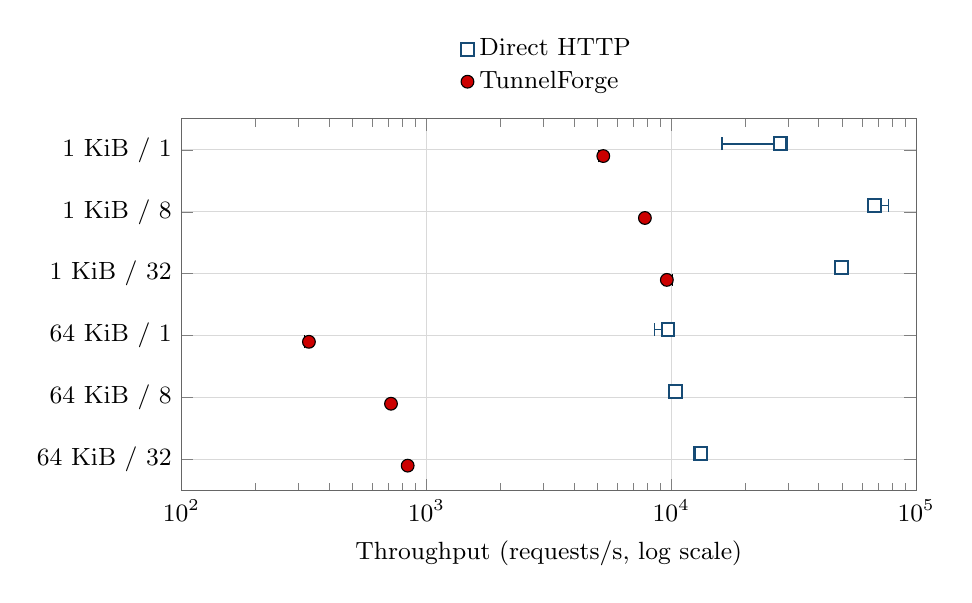
\begin{tikzpicture}
\begin{axis}[
  width=.90\columnwidth,height=6.3cm,
  xmode=log,xmin=100,xmax=100000,
  ymin=.5,ymax=6.5,
  ytick={1,2,3,4,5,6},
  yticklabels={64 KiB / 32,64 KiB / 8,64 KiB / 1,
               1 KiB / 32,1 KiB / 8,1 KiB / 1},
  xtick={100,1000,10000,100000},
  xticklabels={$10^2$,$10^3$,$10^4$,$10^5$},
  xlabel={Throughput (requests/s, log scale)},
  tick label style={font=\small},
  label style={font=\small},
  legend style={font=\small,at={(.5,1.04)},anchor=south,
    legend columns=1,draw=none,cells={anchor=west}},
  grid=major,grid style={black!15},
  axis line style={black!60},
  clip=true]
\addplot+[
  only marks,mark=square*,mark size=2.3pt,color=relayblue,
  mark options={fill=white,line width=.8pt},
  error bars/.cd,x dir=both,x explicit,
  error bar style={line width=.6pt}]
table[row sep=crcr,x=rate,y=pos,x error minus=minus,x error plus=plus] {
rate pos minus plus\\
27855.4 6.10 11738.3 49.4\\
67579.6 5.10 389.5 9619.9\\
49641.7 4.10 2919.3 2273.0\\
9698.4 3.10 1187.0 398.5\\
10395.0 2.10 566.5 347.0\\
13213.6 1.10 618.9 461.4\\
};
\addlegendentry{Direct HTTP}
\addplot+[
  only marks,mark=*,mark size=2.3pt,color=black,
  error bars/.cd,x dir=both,x explicit,
  error bar style={line width=.6pt}]
table[row sep=crcr,x=rate,y=pos,x error minus=minus,x error plus=plus] {
rate pos minus plus\\
5279.3 5.90 210.8 14.2\\
7807.4 4.90 246.8 106.9\\
9595.8 3.90 323.2 536.6\\
331.6 2.90 12.2 5.0\\
717.4 1.90 4.8 4.7\\
839.2 .90 1.6 5.4\\
};
\addlegendentry{TunnelForge}
\end{axis}
\end{tikzpicture}
}
\caption{Throughput by payload and concurrency, identified by each row label.
Markers show median run
throughput; whiskers show observed minimum to maximum ranges over three runs,
not confidence intervals. Different marker shapes remain distinct in grayscale.}
\label{fig:throughput}
\end{figure}

Fig.~\ref{fig:throughput} makes observed variability visible. At 1~KiB and
$C=1$, direct throughput ranged from 16,117.1 to 27,904.8 requests/s, while
tunnel throughput ranged from 5,068.5 to 5,293.5 requests/s. This baseline
variation cautions against interpreting one short run as a stable capacity
estimate. The whiskers summarize repetitions, not population uncertainty.

\subsection{Interpretation of RQ3}
Tunnelled HTTP is consistently slower than direct HTTP in the collected
conditions. It adds relay handling, JSON/Base64 serialization in both
directions, a shared WebSocket path, and another HTTP exchange. Larger bodies
increase representation work and buffering. No CPU, allocation, or pipeline
profiling was performed, so the experiment cannot identify the dominant
mechanism. Binary framing and streaming are plausible improvements requiring
controlled follow-up experiments.

\section{Discussion and Threats to Validity}
\subsection{Design Implications}
The design is a compact example of reconstructing HTTP over an outbound
connection. Tests establish sampled representation, correlation, and failure
behavior; measurements make the local cost visible. Inspectability is useful
for explaining how Go values become JSON and reconstructed requests, but a
teaching benefit is a rationale, not a measured learning outcome.

The design separates connection liveness from request completion: a healthy
socket does not ensure that an application request will finish, so independent
deadlines are necessary. Likewise, client registration does not establish
ownership of every request ID; the pending map records that relationship.
These distinctions explain the separate heartbeat, timeout, and correlation
mechanisms.

\subsection{Internal and External Validity}
Short runs, imperfect mode-order balancing, incomplete concurrent connection
warm-up, and background load limit internal validity. The generator shares
CPU and memory with all services and can affect throughput. Timings include
body reading and validation, so they are application-observed round trips,
not transport-only measurements. The artifact records these choices for
reproduction but does not remove their effects.

One host, runtime, echo operation, two body sizes, and three concurrency levels
cannot represent Internet traffic. There is no cross-machine trial, mobile
network, loss injection, WAN delay, NAT traversal test, TLS measurement, or
long-duration soak test. These data cannot establish public-cloud performance,
maximum capacity, or superiority to ngrok or frp. Three repetitions justify
descriptive medians and ranges, not statistical-significance claims.

\subsection{Implementation Limitations}
All relay state resides in one process. Restart invalidates URLs; multiple
replicas would require connection-aware routing or inter-relay forwarding.
The pending-request limit is not a user quota, and the shared token does not
provide per-user identity, revocation, accounting, or public-caller policies.

Path routing can require changes for root-relative links, absolute redirects,
cookie paths, and virtual-host assumptions. Bodies are fully buffered; the
implementation does not rewrite arbitrary content or support server-sent
events, tunnelled WebSocket upgrades, raw TCP, or gRPC streaming. Public
HTTPS/WSS deployment was not evaluated. A Docker image build was blocked by
a registry certificate mismatch; native execution is the measured artifact.

\subsection{Future Work}
First deploy to a reachable TLS endpoint and measure from another network.
Next, profile CPU and allocations, and compare JSON/Base64 against binary
frames while holding other factors constant. Streaming, cancellation-aware
backpressure, and fair admission could support larger bodies. Broader hosting
would require per-user credentials, caller access policies, rate controls,
and connection-aware multi-relay routing.

\section{Conclusion}
TunnelForge implements a reverse HTTP tunnel in Go using a versioned JSON
protocol over WebSocket. Temporary registration, ownership-aware request
matching, bounded concurrency, cancellation, and connection recovery are
integrated in one inspectable implementation. Functional tests and 9,216
checked loopback requests support correctness for the evaluated scenarios.
Local overhead is substantial relative to direct HTTP, especially for larger
bodies, motivating more efficient framing and buffering. The artifact supports
reproducible local demonstrations; Internet deployment, broad compatibility,
and production capacity remain unverified.

% Self-contained bibliography: Overleaf needs no .bib file or BibTeX step.
\begin{thebibliography}{00}
\bibitem{websocket}
I.~Fette and A.~Melnikov, ``The WebSocket Protocol,'' IETF, RFC~6455,
Dec. 2011, doi: 10.17487/RFC6455.
[Online]. Available: \url{https://www.rfc-editor.org/rfc/rfc6455}

\bibitem{http}
R.~Fielding, M.~Nottingham, and J.~Reschke, Eds., ``HTTP Semantics,''
IETF, RFC~9110, Jun. 2022, doi: 10.17487/RFC9110.
[Online]. Available: \url{https://httpwg.org/specs/rfc9110.html}

\bibitem{ngrok}
ngrok, ``What is ngrok?,'' Documentation, accessed Oct. 29, 2026.
[Online]. Available: \url{https://ngrok.com/docs/about}

\bibitem{frp}
fatedier and contributors, ``frp: A fast reverse proxy,'' GitHub repository,
accessed Oct. 29, 2026.
[Online]. Available: \url{https://github.com/fatedier/frp}

\bibitem{json}
T.~Bray, Ed., ``The JavaScript Object Notation (JSON) Data Interchange
Format,'' IETF, RFC~8259, Dec. 2017, doi: 10.17487/RFC8259.
[Online]. Available: \url{https://www.rfc-editor.org/rfc/rfc8259}

\bibitem{base64}
S.~Josefsson, ``The Base16, Base32, and Base64 Data Encodings,'' IETF,
RFC~4648, Oct. 2006, doi: 10.17487/RFC4648.
[Online]. Available: \url{https://www.rfc-editor.org/rfc/rfc4648}

\bibitem{gojson}
The Go Authors, ``Package encoding/json,'' Go package documentation,
accessed Oct. 29, 2026.
[Online]. Available: \url{https://pkg.go.dev/encoding/json}

\bibitem{gorilla}
Gorilla WebSocket contributors, ``Package websocket,'' Go package
documentation, accessed Oct. 29, 2026.
[Online]. Available: \url{https://pkg.go.dev/github.com/gorilla/websocket}

\bibitem{race}
The Go Authors, ``Data Race Detector,'' Go documentation, accessed Oct. 29,
2026. [Online]. Available: \url{https://go.dev/doc/articles/race_detector}
\end{thebibliography}

\end{document}
